\documentclass[a4paper, 12pt]{report}
\setlength{\headheight}{15.71667pt}
\addtolength{\topmargin}{-3.71667pt}
\usepackage[spanish]{babel}
\usepackage[utf8]{inputenc}
\usepackage{graphicx}
\usepackage{hyperref}
\usepackage{fancyhdr}
\usepackage{amsmath}
\usepackage{listings}
\usepackage{geometry}

\geometry{left=2.5cm, right=2.5cm, top=2.5cm, bottom=2.5cm}
\hypersetup{
	colorlinks=true,
	linkcolor=blue,
	urlcolor=blue,
}

% Encabezado y pie de página
\pagestyle{fancy}
\fancyhf{}
\fancyhead[L]{Documentación}
\fancyhead[R]{\leftmark}
\fancyfoot[C]{\thepage}

% Datos de portada
\newcommand{\portada}{
    \begin{titlepage}
        \centering
        \vspace*{1cm}
        
        
\includegraphics[width=0.2\textwidth]{./images/escudo_principal.png} \hfill
        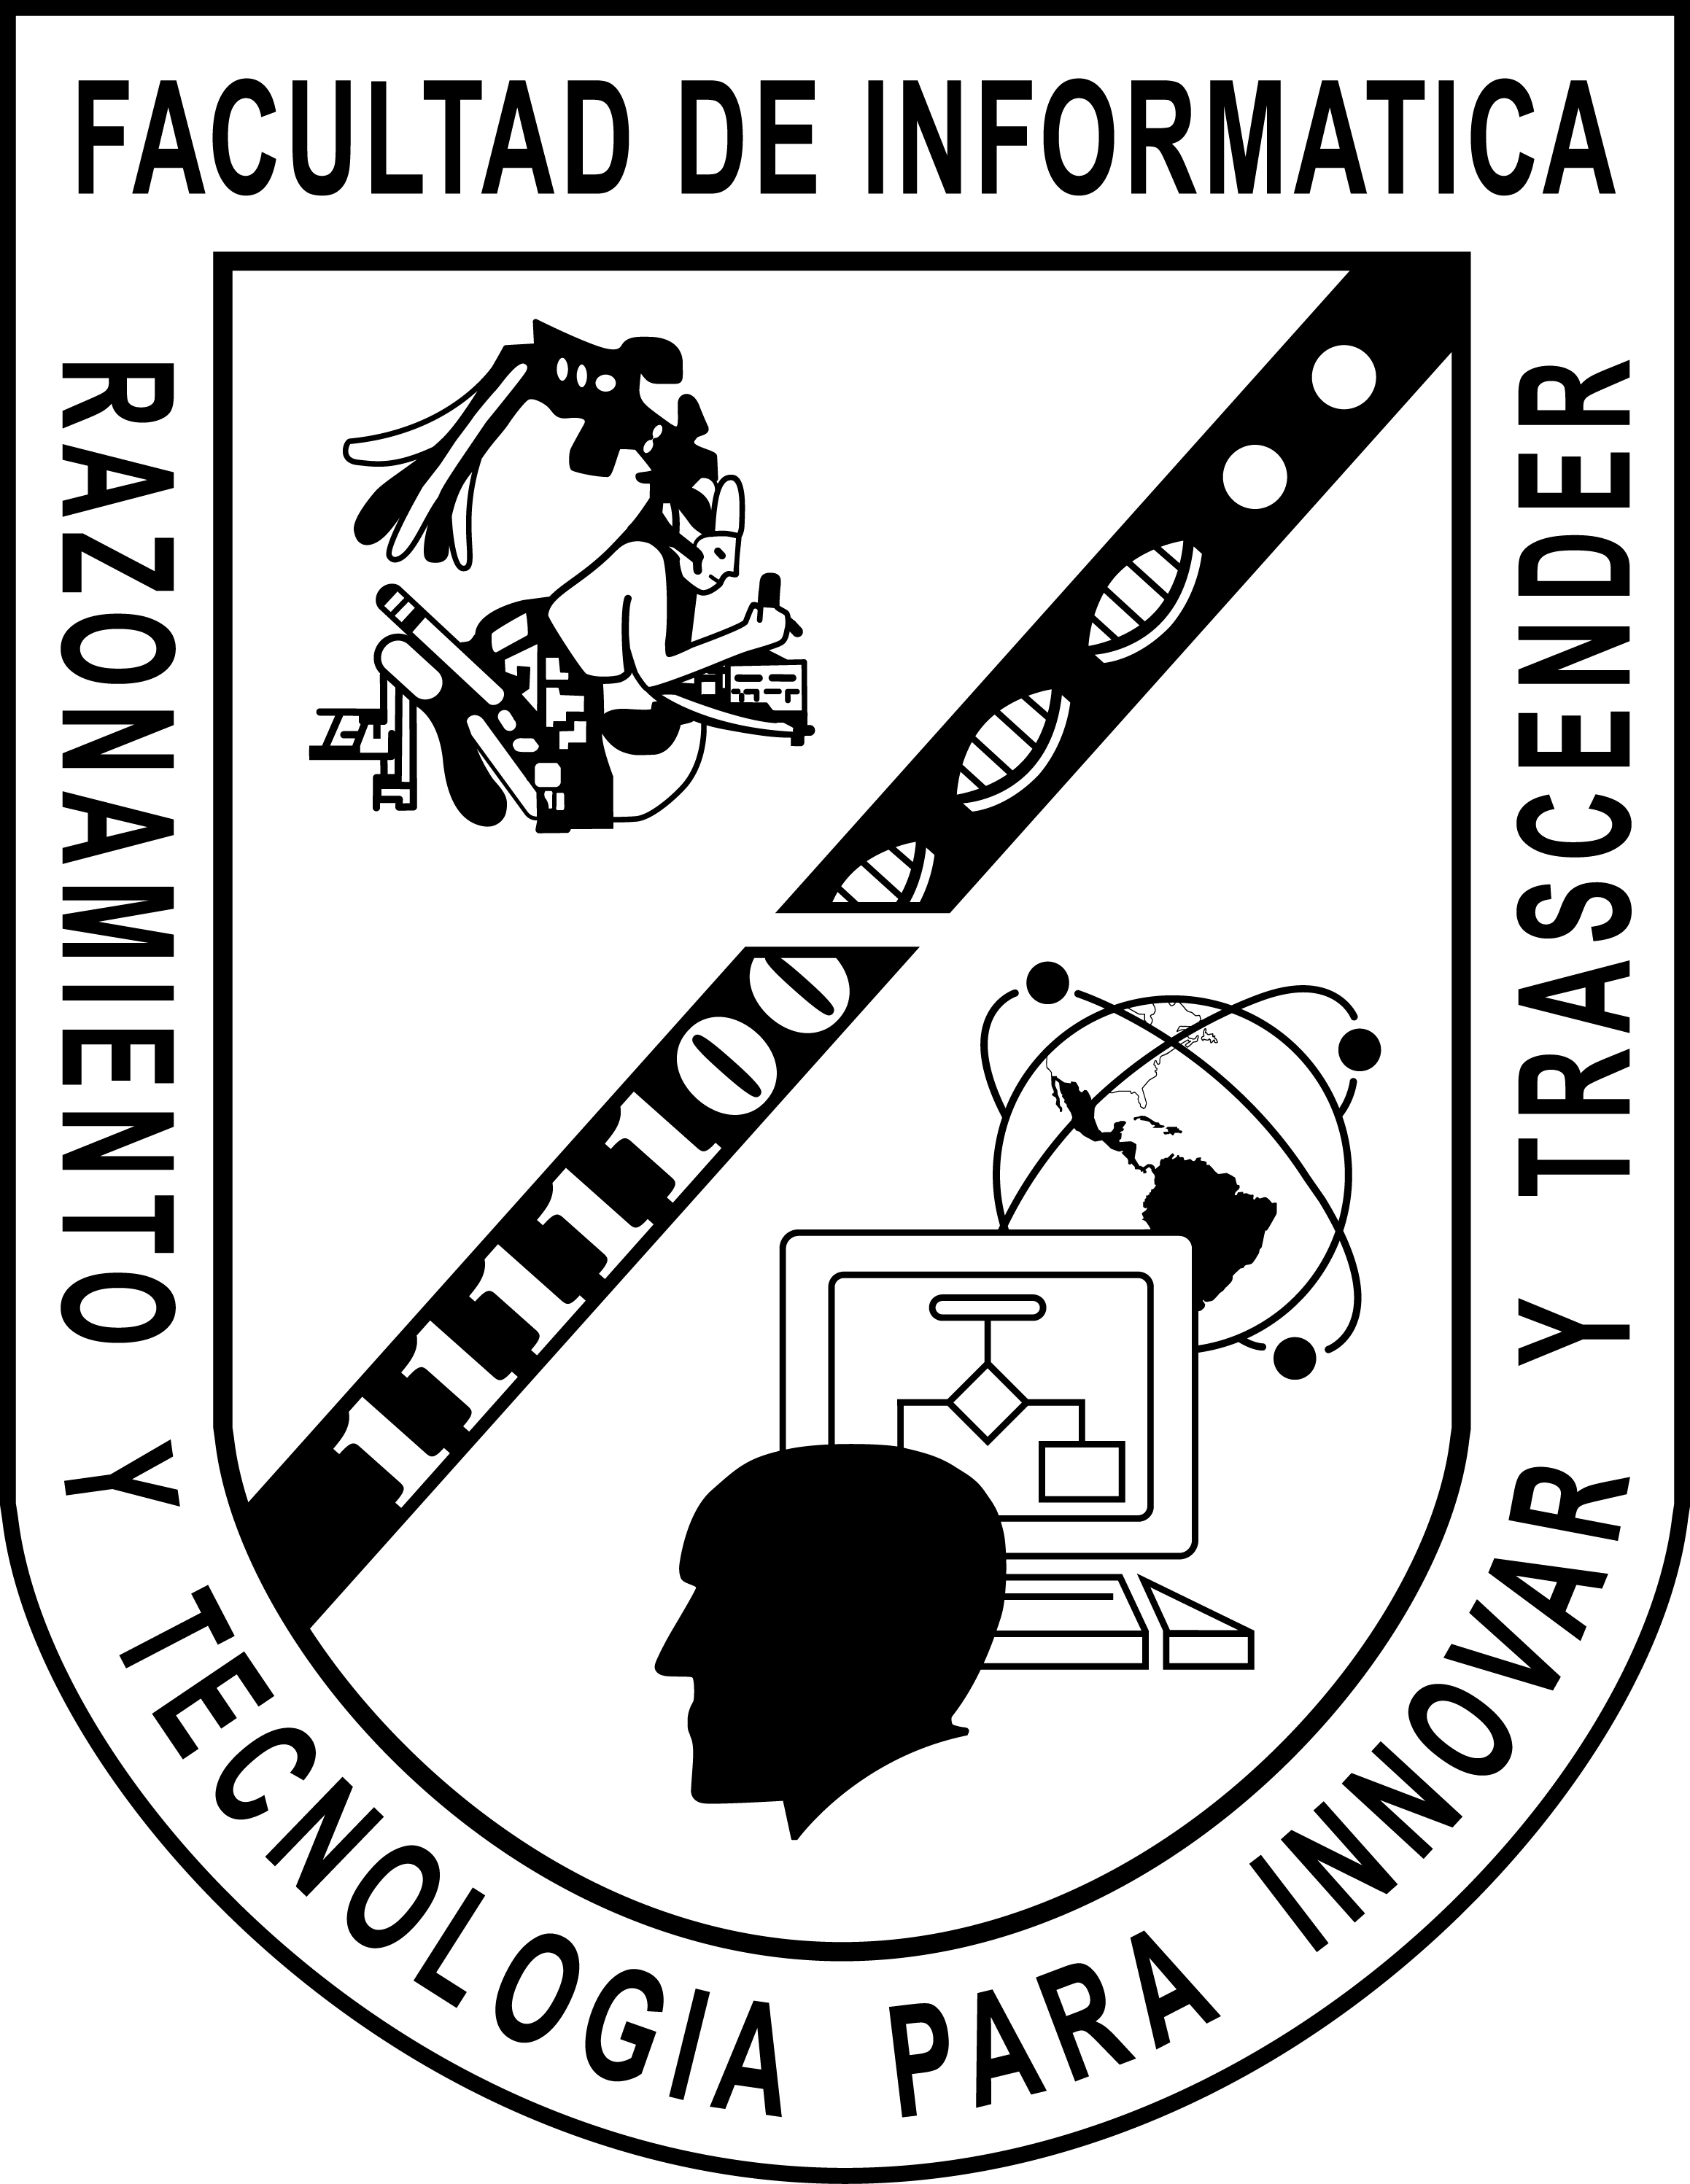
\includegraphics[width=0.2\textwidth]{./images/escudo_secundario.png}
        
        \vspace{2cm}
        
        {\Huge \textbf{Proyecto Final\\Ingeniería de Requerimientos}}
        
        \vspace{1.5cm}
        
        {\Large Documentación del Proyecto}
        
        \vspace{2cm}
        
        \textbf{Participantes:}
        
        \vspace{0.5cm}
        \begin{center}
				David Mata Guerra\\
				Alejandro Macías Fonseca\\
				Alexis Emilio Cárdenas Camacho \\
				Gabriel Juárez Ramírez \\
		\end{center}
        
        \vfill
        
        {\Large Universidad Autónoma de Querétaro}
        
        \vspace{0.5cm}
        
        {\Large \today}
        
    \end{titlepage}
}

\begin{document}
	\portada
	\tableofcontents
	\newpage
	
	% Capítulo 1 - Descripción General del Proyecto
	\chapter{Descripción General del Proyecto}
\section{Resumen}
El propósito de este proyecto es crear una herramienta de tareas, la cual pueda crear, editar, eliminar y marcar como completadas
las tareas que el usuario desee. Además, se podrá visualizar las tareas que se han completado y las que están pendientes.

\section{Alcance y Limitaciones}
Alcances del proyecto:
\begin{itemize}
  \item Gestionar el proyecto mediante la herramienta JIRA utilizando la metodología Scrum.
  \item Desarrollar un prototipado con todas las funcionalidades que se dean implementar en Figma.
  \item Hacer uso un repositorio en GitHub para el control de versiones de el frontend.
  \item Hacer uso repositorio en GitHub para el control de versiones de el backend.
  \item Crear un diagrama relacional de la base de datos.
  \item Crear una base de datos con la estructura del diagrama relacional.
  \item Desarrollar la aplicación.
  \item Lanzar la aplicación en un servidor.
  \item Realizar test a la aplicación.
  \item Desglosar los pasos del proyecto en una presentación.
\end{itemize}

Limitaciones del proyecto:
\begin{itemize}
  \item El desarrollo de el proyecto tiene un tiempo limitado (3 semanas y 4 días).
  \item El proyecto no busca fines lucrativos.
  \item El proyecto se encuentra limitado a la creación de tareas.
\end{itemize}


\section{Justificación}
El proyecto surge en base a un proyecto final solicitado en la clase de Ingeniería de Requerimientos
de la Universidad Autónoma de Querétaro. La idea de crear un gestor de tareas es con la finalidad de poner 
a prueba los conocimientos adquiridos en la materia y en la carrera.

	% Capítulo 2 - Especificación de Requisitos
	\chapter{Especificación de Requerimientos}
\section{Requerimientos Funcionales}
\begin{itemize}
  \item Gestión de tareas:
    \begin{itemize}
      \item Crear tareas.
      \item Editar tareas.
      \item Eliminar tareas.
      \item Marcar tareas como completadas.
      \item Establecer fechas límite para las tareas.
    \end{itemize}
  \item Visualización de tareas:
    \begin{itemize}
      \item Interfaz intuitiva y práctica de utilizar.
      \item El usuario pueda reconocer todos los cambios realizados de manera visual.
    \end{itemize}
    \section{Stakeholders}
    \begin{itemize}
        \item Desarrolladores.
        \item Usuarios.
        \item Profesor.
    \end{itemize}
\end{itemize}
\section{Reglas de Negocio}
\begin{enumerate}[start=1, label={RN\arabic*.}]
  \item Las tareas deben de pertenecer a una persona \label{rn:user}
  \item Las tareas deben de tener un nombre \label{rn:nombre}
  \item Las tareas pueden tener una descripci\'on \label{rn:desc}
  \item Las tareas pueden tener una fecha \label{rn:fecha}
  \item Las tareas disponen de dos estados \label{rn:estado}
    \begin{itemize}
      \item Sin completar
      \item Completado
    \end{itemize}
  \item Las tareas pueden tener 2 niveles de prioridades. \label{rn:prioridad}
    \begin{itemize}
      \item Baja
      \item Alta
    \end{itemize}
  \item Las tareas pueden ser recurrentes
\end{enumerate}
	\section{Casos de Uso}
	\begin{longtable}[c]{p{3cm}p{5cm}p{4cm}p{2cm}}
  \endfirsthead
  \endhead
  \endfoot
  \hline
  ID y nombre & CU-1. Crear una tarea & & \\
  \hline
  Creado por: & Alejandro & Fecha de creaci\'on & 24-11-05\\
  \hline
  Actor principal: & Usuario final & Actores secundarios: & Base de datos, aplicaci\'on principal\\
  \hline
  Descripci\'on & \multicolumn{3}{p{11cm}}{El usuario final especificar\'a una tarea a crear con el bot\'on para crear una nueva tarea. Tendr\'a que especificar el nombre de la tarea (obligatorio), una descripci\'on (opcional) y una fecha de la tarea (opcional)}\\
  \hline
  Trigger: & \multicolumn{3}{p{11cm}}{El usuario final indica que quiere crear una tarea con el bot\'on especificado}\\
  \hline
  Precondiciones: & \multicolumn{3}{p{11cm}}{$\bullet$ PRE-1. El usuario est\'a registrado en la base de datos}\\
		  & \multicolumn{3}{p{11cm}}{$\bullet$ PRE-2. El usuario cuenta con conexi\'on a internet para acceder al sistema}\\
  \hline
  Postcondiciones: & \multicolumn{3}{p{11cm}}{$\bullet$ POST-1. La tarea ser\'a guardada en la base de datos}\\
		   & \multicolumn{3}{p{11cm}}{$\bullet$ POST-2. La tarea ser\'a mostrada en la p\'agina principal del usuario}\\
  \hline
  Flujo normal: & \multicolumn{3}{p{11cm}}{\textbf{1.0. Crear una tarea}}\\
		& \multicolumn{3}{p{11cm}}{$\bullet$ El usuario final pide al sistema crear una nueva tarea mediante la aplicaci\'on}\\
		& \multicolumn{3}{p{11cm}}{$\bullet$ La aplicaci\'on despliega los campos a llenar para la tarea}\\
		& \multicolumn{3}{p{11cm}}{$\bullet$ Una vez llenados los campos, el usuario interact\'ua con la aplicaci\'on para guardar la tarea}\\
		& \multicolumn{3}{p{11cm}}{$\bullet$ La tarea es enviada a la base de datos del sistema y la valida}\\
  \hline
  Flujo alternativo: & \multicolumn{3}{p{11cm}}{\textbf{1.1. Crear una tarea anidada}}\\
		     & \multicolumn{3}{p{11cm}}{$\bullet$ Al seleccionar una tarea, la aplicaci\'on le mostrar\'a al usuario distintos campos para editar, en uno de ellos, el agregar tareas anidadas}\\
		     & \multicolumn{3}{p{11cm}}{$\bullet$ Al seleccionar el campo, se desplegar\'a un campo donde el usuario dar\'a el nombre de la tarea, junto con una opci\'on para guardar la tarea}\\
		     & \multicolumn{3}{p{11cm}}{$\bullet$ Al indicarle el usuario a la aplicaci\'on que quiere guardar la tarea anidada, esta enviar\'a al sistema que se quiere crear una tarea anidada, pas\'andole el identificador de la tarea anidada, junto con el identificador de la tarea padre como campo}\\
		     & \multicolumn{3}{p{11cm}}{$\bullet$ El sistema guarda la tarea anidada en la base de datos}\\
  \hline
  Excepciones: & \multicolumn{3}{p{11cm}}{\textbf{1.0.E1. La tarea ya ha sido creada}}\\
	       & \multicolumn{3}{p{11cm}}{$\bullet$ Si la validaci\'on de la base de datos encuentra que la tarea ya ha sido creada, arroja un error}\\
	       & \multicolumn{3}{p{11cm}}{$\bullet$ La aplicaci\'on escucha si la base de datos arroj\'o el error, y muestra al usuario que la tarea ya ha sido creada}\\
	       & \multicolumn{3}{p{11cm}}{$\bullet$ El usuario no podr\'a guardar la tarea hasta que el campo del t\'itulo sea cambiado}\\
  \hline
  Prioridad: & \multicolumn{3}{p{11cm}}{Alta}\\
  \hline
  Frecuencia de uso: & \multicolumn{3}{p{11cm}}{Aproximadamente de 1 a 5 veces por d\'ia por usuario}\\
  \hline
  Reglas de negocio: & \multicolumn{3}{p{11cm}}{Por definir}\\
  \hline
  Informaci\'on adicional: & \multicolumn{3}{p{11cm}}{La aplicaci\'on deber\'a de mostrar en una ventana emergente los campos a llenar}\\
  \hline
  Asumciones: & \multicolumn{3}{p{11cm}}{Las tareas subidas no se tomar\'an como completadas}\\
  \hline
\end{longtable}
\vspace{1em}
\begin{longtable}[c]{p{3cm}p{5cm}p{4cm}p{2cm}}
  \endfirsthead
  \endhead
  \endfoot
  \hline
  ID y nombre & \multicolumn{3}{p{11cm}}{CU-2. Eliminar una tarea}\\
  \hline
  Creado por: & Alejandro & Fecha de creaci\'on & 24-11-05\\
  \hline
  Actor principal: & Usuario final & Actores secundarios: & Base de datos, aplicaci\'on principal\\
  \hline
  Descripci\'on & \multicolumn{3}{p{11cm}}{El usuario eliminar\'a de sus tareas una tarea especificada por este por medio de la aplicaci\'on.}\\
  \hline
  Trigger: & \multicolumn{3}{p{11cm}}{El usuario final indica que quiere eliminar una tarea con el bot\'on especificado}\\
  \hline
  Precondiciones: & \multicolumn{3}{p{11cm}}{PRE-1. El usuario est\'a registrado en la base de datos}\\
		  & \multicolumn{3}{p{11cm}}{PRE-2. El usuario cuenta con conexi\'on a internet para acceder al sistema}\\
		  & \multicolumn{3}{p{11cm}}{PRE-3. El usuario cuenta con al menos una tarea registrada en la base de datos}\\
  \hline
  Postcondiciones: & \multicolumn{3}{p{11cm}}{POST-1. La tarea ser\'a eliminada permanentemente en la base de datos}\\
		   & \multicolumn{3}{p{11cm}}{POST-2. La tarea dejar\'a de ser mostrada mostrada en la p\'agina principal del usuario}\\
  \hline
  Flujo normal: & \multicolumn{3}{p{11cm}}{\textbf{2.0. Eliminar una tarea}}\\
		& \multicolumn{3}{p{11cm}}{$\bullet$ El usuario final pide al sistema eliminar una tarea seleccionada mediante la aplicaci\'on}\\
		& \multicolumn{3}{p{11cm}}{$\bullet$ La aplicaci\'on despliega una ventana emergente con un mensaje de que quiere corroborar eliminar la tarea, junto con dos opciones, las cuales son ``Cancelar'' y ``Confirmar''. En caso de seleccionar ``Cancelar'', el sistema no borra la tarea y la ventana emergente desaparece}\\
		& \multicolumn{3}{p{11cm}}{$\bullet$ Una vez confirmada la elecci\'on, la aplicaci\'on env\'ia la petici\'on a la base de datos de eliminar la tarea seleccionada}\\
		& \multicolumn{3}{p{11cm}}{$\bullet$ La tarea es eliminada de la base del datos del sistema}\\
  \hline
  Flujo alternativo: & \multicolumn{3}{p{11cm}}{\textbf{2.1. Eliminar m\'ultiples tareas}}\\
	       & \multicolumn{3}{p{11cm}}{$\bullet$ El usuario mediante la opci\'on de seleccionar m\'ultiples tareas que provee la aplicaci\'on, escoge distintas tareas destinadas a eliminar}\\
	       & \multicolumn{3}{p{11cm}}{$\bullet$ El usuario utiliza la implementaci\'on de eliminar tarea que provee la aplicaci\'on para eliminar las tareas seleccionadas previamente}\\
	       & \multicolumn{3}{p{11cm}}{$\bullet$ La aplicaci\'on env\'ia al sistema los identificadores de las tareas a eliminar}\\
	       & \multicolumn{3}{p{11cm}}{$\bullet$ El sistema hace la petici\'on a la base de datos para eliminar los registros de las tareas especificadas}\\
	       & \multicolumn{3}{p{11cm}}{$\bullet$ Las tareas son eliminadas de la base de datos}\\
  \hline
  Prioridad: & \multicolumn{3}{p{11cm}}{Alta}\\
  \hline
  Frecuencia de uso: & \multicolumn{3}{p{11cm}}{Aproximadamente de 1 a 2 veces por d\'ia por usuario}\\
  \hline
  Reglas de negocio: & \multicolumn{3}{p{11cm}}{Por definir}\\
  \hline
  Informaci\'on adicional: & \multicolumn{3}{p{11cm}}{La aplicaci\'on deber\'a de mostrar en una ventana emergente el mensaje de confirmaci\'on}\\
  \hline
  Asumciones: & \multicolumn{3}{p{11cm}}{El usuario tiene al menos una tarea registrada}\\
  \hline
\end{longtable}

\begin{longtable}[c]{p{3cm}p{5cm}p{4cm}p{2cm}}
  \endfirsthead
  \endhead
  \endfoot
  \hline
  ID y nombre & \multicolumn{3}{p{11cm}}{CU-3. Editar una tarea}\\
  \hline
  Creado por: & Alejandro & Fecha de creaci\'on & 24-11-06\\
  \hline
  Actor principal: & Usuario final & Actores secundarios: & Base de datos, aplicaci\'on principal\\
  \hline
  Descripci\'on & \multicolumn{3}{p{11cm}}{El usuario podr\'a editar una tarea por medio de la aplicaci\'on.}\\
  \hline
  Trigger: & \multicolumn{3}{p{11cm}}{El usuario final indica que quiere editar una tarea al entrar en una tarea}\\
  \hline
  Precondiciones: & \multicolumn{3}{p{11cm}}{PRE-1. El usuario est\'a registrado en la base de datos}\\
		  & \multicolumn{3}{p{11cm}}{PRE-2. El usuario cuenta con conexi\'on a internet para acceder al sistema}\\
		  & \multicolumn{3}{p{11cm}}{PRE-3. El usuario cuenta con al menos una tarea registrada en la base de datos}\\
  \hline
  Postcondiciones: & \multicolumn{3}{p{11cm}}{POST-1. La tarea ser\'a editada en la base de datos}\\
		   & \multicolumn{3}{p{11cm}}{POST-2. La tarea ser\'a mostrada con su nueva informaci\'on en la p\'agina principal del usuario}\\
  \hline
  Flujo normal: & \multicolumn{3}{p{11cm}}{\textbf{3.0. Editar una tarea}}\\
		& \multicolumn{3}{p{11cm}}{$\bullet$ El usuario final selecciona una tarea}\\
		& \multicolumn{3}{p{11cm}}{$\bullet$ La aplicaci\'on despliega una ventana con los datos de la tarea, dej\'andolos abiertos para editarlos}\\
		& \multicolumn{3}{p{11cm}}{$\bullet$ Una vez el usuario haya editado la tarea a voluntad, el usuario interact\'ua con la aplicaci\'on en un bot\'on dedicado para guardar la tarea}\\
		& \multicolumn{3}{p{11cm}}{$\bullet$ La aplicaci\'on env\'ia al sistema que se quieren actualizar los datos de la tarea especificada}\\
		& \multicolumn{3}{p{11cm}}{$\bullet$ El sistema valida la actualizaci\'on}\\
		& \multicolumn{3}{p{11cm}}{$\bullet$ El sistema actualiza la informaci\'on de la tarea especificada en la base de datos}\\
  \hline
  Excepciones & \multicolumn{3}{p{11cm}}{\textbf{3.0.E1. Renombrar como una tarea ya creada}}\\
	      & \multicolumn{3}{p{11cm}}{$\bullet$ En caso de que el nombre de la tarea ya exista, el sistema arroja un error de que la tarea ya existe.}\\
	      & \multicolumn{3}{p{11cm}}{$\bullet$ La aplicaci\'on atrapa el error, y despliega en una ventana emergente el error.}\\
  \hline
  Prioridad: & \multicolumn{3}{p{11cm}}{Alta}\\
  \hline
  Frecuencia de uso: & \multicolumn{3}{p{11cm}}{Aproximadamente de 1 a 2 veces por d\'ia por usuario}\\
  \hline
  Reglas de negocio: & \multicolumn{3}{p{11cm}}{Por definir}\\
  \hline
  Informaci\'on adicional: & \multicolumn{3}{p{11cm}}{La aplicaci\'on deber\'a de mostrar en una ventana emergente el mensaje de confirmaci\'on}\\
  \hline
  Asumciones: & \multicolumn{3}{p{11cm}}{El usuario tiene al menos una tarea registrada}\\
  \hline
\end{longtable}
 
    
    \section{Historias de Usuario}
    \begin{enumerate}[start=1, label=HU\arabic*.]
        \item Como usuario, quiero poder crear nuevas tareas para organizar y gestionar mis actividades diarias.
        
        \item Como usuario, quiero poder ver una lista de todas mis tareas pendientes para tener una visión clara de lo que necesito hacer.
        
        \item Como usuario, quiero poder marcar las tareas como completadas para llevar un seguimiento de mi progreso.
        
        \item Como usuario, quiero poder establecer fechas límite para mis tareas para asegurarme de cumplir con mis plazos.

        \item Como usuario, quiero poder editar mis tareas para poder hacer cambios en ellas si es necesario.
    \end{enumerate}
\section{Requerimientos No Funcionales}
\begin{itemize}
  \item Rendimiento:
    \begin{itemize}
      \item No debe de haber errores en la logica de programacion.
      \item La aplicación debe de ser rápida y eficiente.
    \end{itemize}
\end{itemize}

	% Capítulo 3 - Análisis y Diseño del Sistema
	\chapter{Análisis y Diseño del Sistema}	

\section{Frontend}

\section{Backend}

\subsection{Manejo de rutas y m\'etodos}

\begin{itemize}
  \item \texttt{'/'}.\\
    En la ruta principal, el usuario entrar\'a a la \textit{landing page}, donde se mostrar\'an los objetivos b\'asicos de la aplicaci\'on, y el apartado respectivo para entrar a la aplicaci\'on
  \item \texttt{'/app/:idUser/tasks'}
    \begin{itemize}
      \item \texttt{GET}. Se mostrar\'an todas las tareas que el usuario tenga (mostrar\'a como tareas principales aquellas que no tengan definido su par\'ametro de tarea padre).
      \item \texttt{POST}. La ruta recibir\'a en el formato correspondiente las tareas a crear
    \end{itemize}
\end{itemize}

	% Capítulo 4 - Planificación y Gestión del Proyecto
		\chapter{Planificación y Gestión del Proyecto}
	\section{Cronograma}
	Incluya un cronograma o diagrama de Gantt.
	
	\section{Recursos y Roles}
	Defina los recursos necesarios y los roles del equipo.
	
	\section{Control de Versiones}
	Describa cómo se gestionará el control de versiones.
	

	% Capítulo 5 - Manual de Usuario
		\chapter{Manual de Usuario}
	\section{Guía de Uso}
	Instrucciones para el usuario final.
	
	\section{Resolución de Problemas Comunes}
	Resuelva dudas o problemas frecuentes.
	

	% Capítulo 6 - Manual Técnico o de Mantenimiento
		\chapter{Documentación de Despliegue}
	\section{Instrucciones de Instalación}
	Cómo instalar y desplegar el sistema.
	
	\section{Requisitos de Hardware y Software}
	Describa los requisitos del entorno de producción.
	

	% Capítulo 7 - Registro de Cambios
		\chapter{Registro de Cambios (Changelog)}
	Documente los cambios y versiones del sistema.

\end{document}
